\documentclass[twoside, openany, 12pt, a5paper]{book}
\usepackage{tikz}
\usepackage{multicol}
\usepackage{geometry}
\usepackage{graphicx}
\usepackage{tipa}
\usepackage{blindtext}
\usepackage{fontspec}
\usepackage[t,lf]{spectral}
\usepackage{xpatch}
\include{Cmd}
\include{Lines}
\include{Grid}
%\usepackage[style=authoryear, backend=biber]{biblatex}

\def\leftsym{\DeclareLetter{\CenterVertical}{\Dot{CenterLeft}}}
\def\rightsym{\DeclareLetter{\RightCurveBottomRight}{(4 .2.5}}

\let\cleardoublepage=\clearpage

\newlength{\chaptertopskip}
\setlength{\chaptertopskip}{-50pt}
\makeatletter
\xpatchcmd{\@makechapterhead}{\vspace*{50\p@}}{\vspace*{\chaptertopskip}}{\typeout{Success}}{\typeout{Failure!!!}}
\makeatother

%\addbibresource{Bibliography.bib}
%\nocite{*}
\pagestyle{plain}
\usepackage[markcase=noupper% remove the uppercasing
]{scrlayer-scrpage}
\ohead{}% clear the outer head
\cfoot*{\pagemark}% the pagenumber in the center of the foot, also on plain pages


\title{Atlan: the guide}
\author{The Conlangers}
\date{}
\nocite{*}
\begin{document}
\frontmatter
\begin{titlepage}
\newgeometry{lmargin=20pt, rmargin=20pt}
\begin{center}
{{\fontsize{30}{36}\selectfont \Huge A T L A N}}
\vspace{2cm}

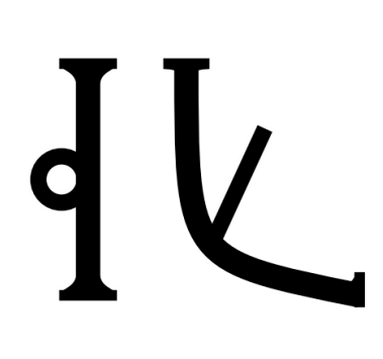
\includegraphics[scale=0.8]{Logo2.jpeg}

\vspace{3cm}
{{\fontsize{30}{36}\selectfont \Large A quick guide}}
\end{center}
\end{titlepage}
\restoregeometry
\blindtext[5]

\mainmatter
\chapter{Introduction}
\Blindtext

\chapter{Need for an IAL}

\Blindtext

\chapter{Phonology}


\Blindtext
\chapter{Writing system}

\Blindtext
\section*{Mathematics and numeric system}

\Blindtext
\section*{Music}

\blindtext[1]

\chapter{Ontology}
\blindtext[3]
\chapter{Lexicon}

\section*{The Story of Babel}

\Blindtext

\section*{AI generation}

\Blindtext

\newgeometry{bmargin=70pt,tmargin=30pt,margin=20pt}
\section*{Atlan - English}
\def\thickness{50pt} \footnotesize
\def\a{\DeclareLetter{\LeftVertical}{\CenterHorizontal}}
\def\b{\DeclareLetter{\CenterHorizontal}{\Dot{Center}}}
\def\c{\DeclareLetter{\ArchBottomRight}{\UpperHorizontal}}
\def\d{\DeclareLetter{\CenterVertical}{\Dot{CenterHeaven}}}


\setlength{\columnsep}{0.7cm}
\begin{multicols}{2} \setlength{\columnsep}{2cm}
	\def\ns{\hspace{-0.2cm}}
	\def\dicentry{\noindent\hspace{-0.1cm}\a\ns\b\ns\c\ns\d \hspace{0.15cm} (\textipa{\bfseries f@"nEtIks}) This is dummy text. The phonetics and the glyphs won't match. I hope this gives a good impression of a dictionary entry. }
\dicentry

\dicentry

\dicentry

\dicentry

\dicentry

\dicentry

\dicentry

\dicentry

\dicentry

\dicentry

\dicentry

\dicentry

\dicentry

\dicentry

\dicentry

\dicentry

\dicentry

\dicentry

\dicentry

\dicentry

\dicentry
\end{multicols}

\newgeometry{tmargin=40pt, bmargin=40pt,margin=20pt}

\setlength{\chaptertopskip}{-20pt}
\makeatletter
\xpatchcmd{\@makechapterhead}{\vspace*{50\p@}}{\vspace*{\chaptertopskip}}{\typeout{Success}}{\typeout{Failure!!!}}
\makeatother



\chapter{English-Atlan}
\def\ns{\hspace{-0.2cm}}
\def\entrytwo{{\noindent \bf sampleword} \hspace{0.15cm} \a\ns\b\ns\c\ns\d \hspace{0.15cm} Some arbitrary explanation of the word. Filler text. \vspace{0.1cm}}
\begin{multicols}{2}
\entrytwo

\entrytwo

\entrytwo

\entrytwo

\entrytwo

\entrytwo

\entrytwo

\entrytwo

\entrytwo

\entrytwo

\entrytwo

\entrytwo

\entrytwo

\entrytwo

\entrytwo

\entrytwo

\entrytwo

\entrytwo

\entrytwo

\entrytwo

\entrytwo

\entrytwo

\entrytwo

\entrytwo

\entrytwo

\entrytwo

\entrytwo

\entrytwo

\entrytwo

\entrytwo


\entrytwo

\entrytwo

\entrytwo

\entrytwo

\entrytwo

\entrytwo

\entrytwo

\entrytwo

\entrytwo

\entrytwo

\entrytwo

\entrytwo

\entrytwo

\entrytwo

\entrytwo

\entrytwo

\entrytwo

\entrytwo

\entrytwo

\entrytwo

\entrytwo

\entrytwo

\entrytwo

\entrytwo

\entrytwo

\entrytwo

\entrytwo

\entrytwo

\entrytwo

\entrytwo

\end{multicols}
\restoregeometry
\chapter{Pragmatics}
\normalsize
\blindtext[1]

\chapter{Translations into Atlan}

\section*{The Story of Babel}
\blindtext[3]
\section*{Alice in Wonderland}
\blindtext[3]
\section*{The Declaration of Universal Human Rights}
\blindtext[3]
\chapter{Practice exercises}
\section{Words and translation}
\newcounter{exercise}
\counterwithin*{exercise}{section}
\newenvironment{exercise}[1][]{%
\stepcounter{exercise}%
\setlength{\parindent}{0pt}%
{\bf \theexercise.~}}%
{\linebreak\noindent}
\def\a{\DeclareLetter{\LeftVertical}{\CenterHorizontal}}
\def\b{\DeclareLetter{\CenterHorizontal}{\Dot{Center}}}
\def\c{\DeclareLetter{\ArchBottomRight}{\UpperHorizontal}}
\def\d{\DeclareLetter{\CenterVertical}{\Dot{CenterHeaven}}}

\begin{exercise}
Recite the Bible in Atlan - without mistakes
\end{exercise}

\begin{exercise}
What is the root of \renewcommand{\thickness}{20pt} \a\ns\b\ns\c\ns\d ? \\ \dotfill 
\end{exercise}

\begin{exercise}\def\sent{\a\ns\b\ns\c\ns\d}
Finish the sentence: \sent \hrulefill \sent
\end{exercise}

\begin{exercise}
	Recommend this book to a friend (or, like, a dozen or something).
\end{exercise}
\renewcommand{\bibname}{\chapter{Sources}}
\bibliography{xampl.bib}
\bibliographystyle{abbrv}

\chapter{Coda}
\blindtext[1]

\chapter{Acknowledgements}
\blindtext[1]

%%%%Flaptekst




\end{document}
